% Intended LaTeX compiler: pdflatex
\documentclass{scrartcl}
    \usepackage{amsmath, amssymb, bm}
		\usepackage[utf8]{inputenc}
		\usepackage[dvipdfmx]{graphicx}
		\usepackage[dvipdfmx]{color}
		\usepackage[backend=biber,bibencoding=utf8]{biblatex}
		\usepackage{url}
		\usepackage{indentfirst}
		\usepackage[normalem]{ulem}
		\usepackage{longtable}
		\usepackage{minted}
		\usepackage{fancyvrb}
    \usepackage[dvipdfmx,colorlinks=false,pdfborder={0 0 0}]{hyperref}
    \usepackage{pxjahyper}
    \usepackage{caption}
\author{elect000}
\date{}
\title{ドキュメント}
\begin{document}

\maketitle
\tableofcontents


\section{Sequence chart}
\label{sec:orgf09497a}
\subsection{login}
\label{sec:org251924d}
\begin{center}
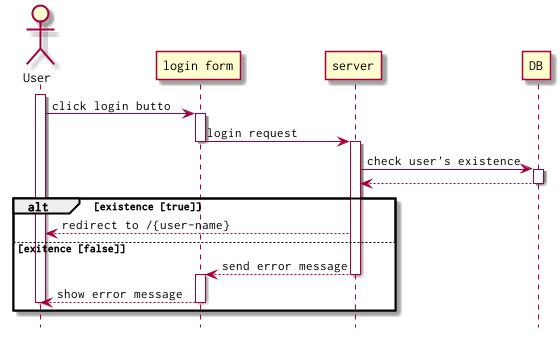
\includegraphics[width=.9\linewidth]{login-seq.png}
\end{center}

\subsection{logout}
\label{sec:org0c01682}
\begin{center}
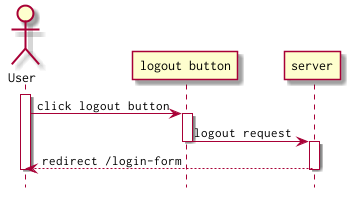
\includegraphics[width=.9\linewidth]{logout-seq.png}
\end{center}
\subsection{select channel}
\label{sec:org89767ef}
\begin{center}
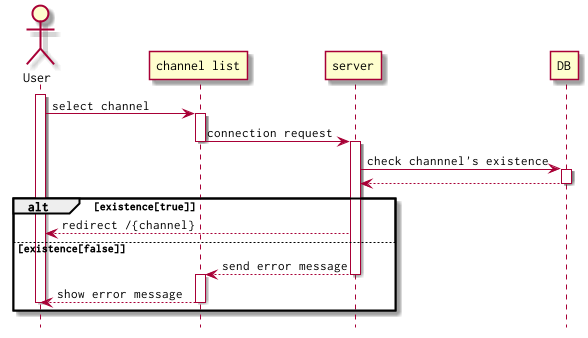
\includegraphics[width=.9\linewidth]{selct-channel-seq.png}
\end{center}
\subsection{make channel}
\label{sec:orgdc3163f}
\begin{center}
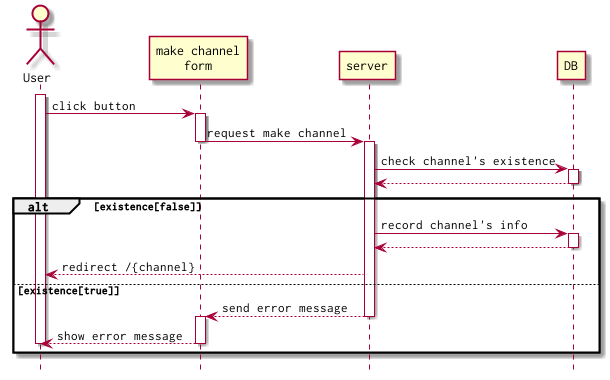
\includegraphics[width=.9\linewidth]{make-channel-seq.png}
\end{center}
\subsection{close channel}
\label{sec:org83ad3ef}
\begin{center}
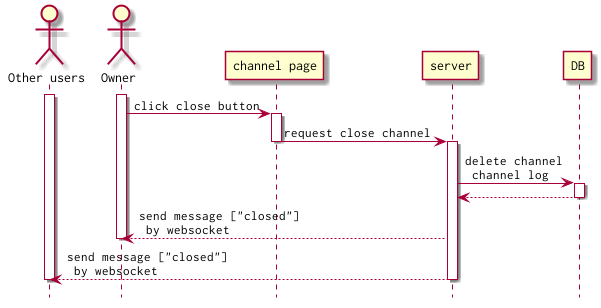
\includegraphics[width=.9\linewidth]{close-channel-seq.png}
\end{center}
\end{document}
